% !Mode:: "TeX:UTF-8"

\begin{frame}{第十七讲、重积分的概念与性质}
	\linespread{1.5}
	\begin{enumerate}
	  \item {\bf 内容与要求}{\b (\S11.1)}
	  \begin{itemize}
	    \item 理解二重积分和三重积分的概念
	    \item 熟练掌握重积分的基本性质
% 	    \item 熟练掌握将二重积分化为累次积分加以计算的方法
% 	    \item 了解最小二乘法
	  \vspace{1em}
	  \end{itemize}
	  \item {\bf  课后作业:}
	  \begin{itemize}
	    \item {\b 习题11.1:4,7(2),8(2)}
% 	    \item {\b 习题11.2:1(4),3(1,3),5(2,4),6(2,3)}
	  \end{itemize}
	\end{enumerate}
\end{frame}

\begin{frame}{什么是重积分}
	\linespread{1.2}\pause 
	\ba{对多元函数的积分运算}\pause 
	
	\bigskip
	\begin{description}
	\item[{\bb 二重积分:}]\pause 
		$$\iint_Df(x,y)\d\sigma$$\pause 
	\item[{\bb 三重积分:}]\pause 
		$$\iiint_{\Omega}f(x,y,z)\d V$$\pause 
	\end{description}
% 	\bigskip
	\ba{关键词:}\pause \alert{微元、\pause 积分区域、\pause 积分次序}
\end{frame}

\section{重积分的概念}

% \begin{frame}{立体的体积}
% 	\linespread{1.2}
% 	\begin{exampleblock}{{\bf 例1:}求以下立体的体积\hfill}
% 		\begin{enumerate}
% 		  \item $x\geq 0,y\geq 0,z\geq 0,x+y+z\leq 2$
% 		  \item $0\leq x\leq 1,0\leq y\leq 1,z\geq 0,x+y+z\leq 2$
% 		\end{enumerate}
% 	\end{exampleblock}\pause 
% 	\begin{itemize}
% 	  \item {\bb 微元法:}$$V=\dint \d V$$\pause 
% 	  \item \ba{ “分割取近似,做和求极限”}
% 	\end{itemize}
% \end{frame}

\begin{frame}{曲顶柱体的体积}
	\linespread{1.2}
	\begin{exampleblock}{{\bf 例1:}求以下立体的体积\hfill}
		$$\Omega:0\leq x\leq 1,0\leq y\leq 1,0\leq z\leq
		3-x^2-y^2$$
	\end{exampleblock}\pause 
	\begin{center}
		\resizebox{!}{4.2cm}{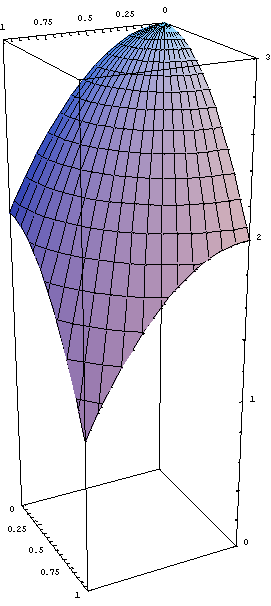
\includegraphics{./images/ch11/volO.pdf}}\quad\pause 
		\resizebox{!}{4.2cm}{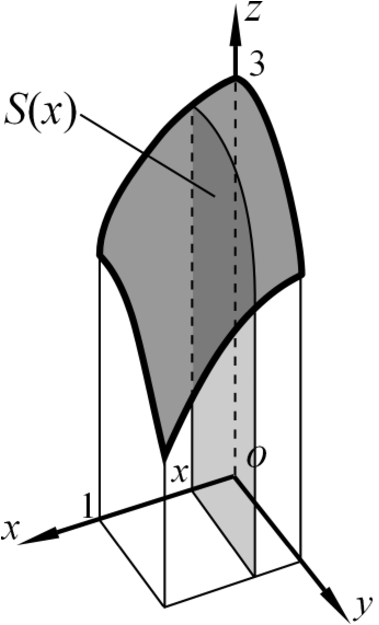
\includegraphics{./images/ch11/volD.pdf}}\quad\pause 
		\resizebox{!}{4.2cm}{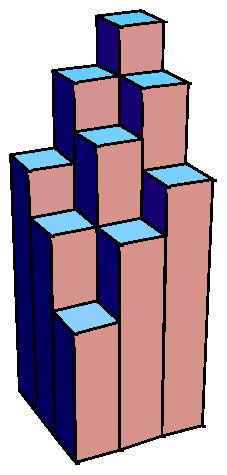
\includegraphics{./images/ch11/volC.pdf}}\quad\pause 
		\resizebox{!}{4.2cm}{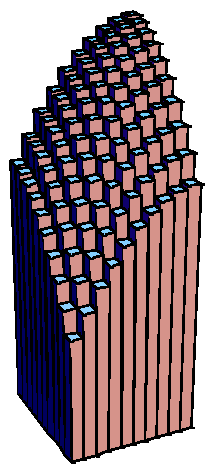
\includegraphics{./images/ch11/volX.pdf}}
	\end{center}
% 	{\bb 微元法:}体积微元
% 	$$dV=S(x)dx$$
% 	截面积:
% 	$$S(x)=\dint_0^1(3-x^2-y^2)dy=\df 83-x^2$$
% 	$$V=\dint_0^1S(x)dx=\df 73$$
\end{frame}

\begin{frame}{立体的质量}
	\linespread{1.2}\pause 
	\begin{exampleblock}{{\bf 例2}\hfill}
		设
		$$\Omega:0\leq x\leq 1,0\leq y\leq 1,0\leq z\leq
		3-x^2-y^2$$
		且$\Omega$内部任一点$(x,y,z)$处的密度为$\rho=1+z$,求$\Omega$的质量。
	\end{exampleblock}
% 	\begin{center}
% 		\resizebox{!}{4.2cm}{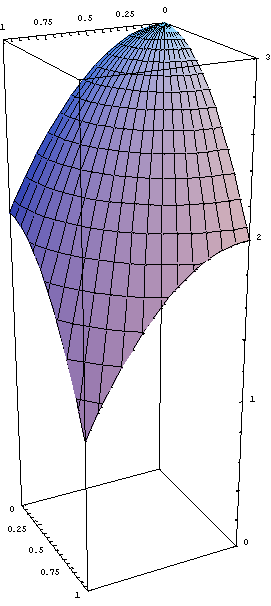
\includegraphics{./images/ch11/volO.pdf}}\quad
% 		\resizebox{!}{4.2cm}{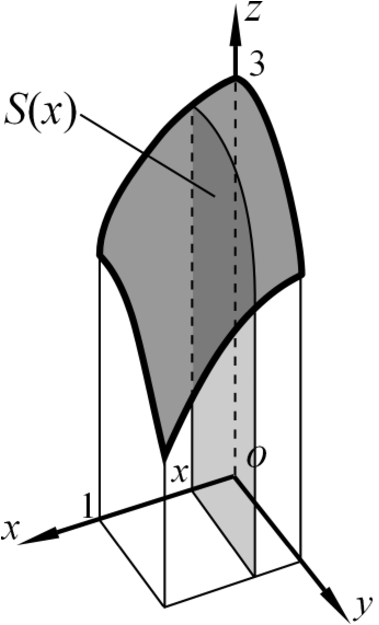
\includegraphics{./images/ch11/volD.pdf}}\quad
% 		\resizebox{!}{4.2cm}{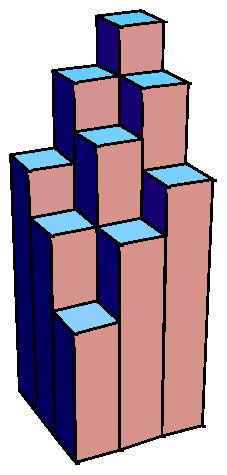
\includegraphics{./images/ch11/volC.pdf}}\quad
% 		\resizebox{!}{4.2cm}{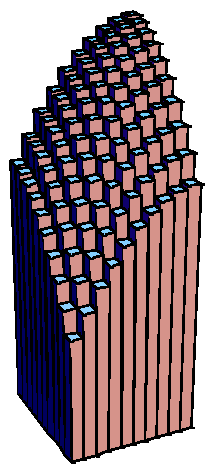
\includegraphics{./images/ch11/volX.pdf}}
% 	\end{center}
% 	{\bb 微元法:}体积微元
% 	$$dV=S(x)dx$$
% 	截面积:
% 	$$S(x)=\dint_0^1(3-x^2-y^2)dy=\df 83-x^2$$
% 	$$V=\dint_0^1S(x)dx=\df 73$$
\end{frame}

\begin{frame}{重积分的定义}
	\linespread{1.2}\pause 
	\begin{block}{{\bf 定义11.1.1-2}\hfill}
% 		设$f(x,y)$在区域$D$内有定义
% 		\begin{enumerate}
% 		  \item {\bb 分割:}将$D$分割成互不相交的小区域
% 		  \vspace{-1ex}
% 		  	$$\Delta\sigma_i,i=1,2,\ldots,n$$
% 	  	  \item {\b 取近似:}在每个$\Delta\sigma_i$中任取一点$(\xi_i,\eta_i)$  
% 	  	  \item {}
% 		\end{enumerate}
		\begin{enumerate}
		  \item {\bb 二重积分:}\pause 
		  $$\iint_Df(x,y)\d\sigma=\lim_{d(T)\to
		  0}\sum_{i=1}^nf(\xi_i,\eta_i)\Delta\sigma_i$$\pause 
		  \item {\bb 三重积分:}\pause 
		  $$\iiint_{\Omega}f(x,y,z)\d V=\lim_{d(T)\to
		  0}\sum_{i=1}^nf(\xi_i,\eta_i,\zeta_i)\Delta V_i$$
		\end{enumerate}
	\end{block}
\end{frame}

\section{重积分的性质}

\begin{frame}{重积分的性质}
	\linespread{1.2}\pause 
	\begin{enumerate}
	  \item {\bf 线性性}\pause 
	  \item {\bf 区域可加性}\pause 
	  \item {\bf 保号性I:}\pause 若在$D$上,$f(x,y)\geq 0$,则
	  $$\iint_Df(x,y)\d\sigma\geq 0$$\pause 
	  \item {\bf 保号性II:}\pause 若$f(x,y)$在$D$上连续,则
	  $$\iint_Df(x,y)\d\sigma=0$$
	  当且仅当在$D$上恒有$f(x,y)=0$
	\end{enumerate}
\end{frame}

\begin{frame}{保号性的推广}
	\linespread{1.2}\pause 
% 	{\bf 推论:}
	\begin{itemize}
	  \item 若在$D$上,$f(x,y)\leq g(x,y)$,则
	  $$\iint_Df(x,y)\d\sigma\leq\iint_Dg(x,y)\d\sigma$$\pause 
	  \vspace{-1em}
	  \item $$\left|\iint_Df(x,y)\d\sigma\right|\leq\iint_D|f(x,y)|\d\sigma$$\pause 
	  \item 设$M,m$分别为$f(x,y)$在$D$上的最大和最小值,$D$的面积为$A$,则
	  $$mA\leq\iint_Df(x,y)\d\sigma\leq MA$$
	\end{itemize}
\end{frame}

\begin{frame}{积分中值定理}
	\linespread{1.2}\pause 
	\begin{block}{{\bf 定理}\hfill}
		设函数$f(x,y)$在有界闭区域$D$上连续非负,$D$的面积为$A$,则存在
		$(\xi,\eta)\in D$,使得
		$$\iint_Df(x,y)\d\sigma=f(\xi,\eta)A$$
	\end{block}
	\bigskip\pause 
% 	\hrule
% 	\bigskip
	\centerline{\ba{通过与定积分的类比,理解重积分的概念与性质}}
\end{frame}

% \section{二重积分的计算}
% 
% \begin{frame}{二重积分与累次积分}
% 	\linespread{1.2}\pause 
% 	{\bb 二重积分:}
% 	$$\alert{\iint_Df(x,y)d\sigma=\lim_{d(T)\to
% 	  0}\sum_{i=1}^nf(\xi_i,\eta_i)\Delta\sigma_i}$$
% 	\pause 令$d\sigma=dydx$,\pause 且
% 	$$D=\{x_1\leq x\leq x_2,\varphi_1(x)\leq y\leq \varphi_2(x)\}$$
% 	\pause 则二重积分可化为{\bb 累次积分:}
% 	$$\alert{\iint_Df(x,y)d\sigma=\int_{x_1}^{x_2}
% 	\int_{\varphi_1(x)}^{\varphi_2(x)}f(x,y)dydx}$$
% \end{frame}
% 
% \begin{frame}{积分区域与累次积分的次序}
% 	\linespread{1.2}\pause 
% 	\ba{将二重积分化为累次积分时,不同的积分次序,对应于不同的积分区域表示方法}\pause 
% 	\begin{exampleblock}{{\bf 例4}\hfill}
% 		计算
% 		$$\iint_Dxyd\sigma,$$
% 		其中$D$为抛物线$y=x^2$和$x=y^2$所围区域。
% 	\end{exampleblock}\pause 
% 	\begin{itemize}
% 	  \item {\bb 先$x$后$y$:}$D:y^2\leq x\leq\sqrt y,\,0\leq y\leq 1$\pause 
% 	  \item {\bb 先$y$后$x$:}$D:x^2\leq y\leq\sqrt x,\,0\leq x\leq 1$
% 	\end{itemize}
% \end{frame}
% 
% \begin{frame}{二重积分的计算}
% 	\linespread{1.2}\pause 
% 	\begin{enumerate}
% 	  \item {\bb 画图:}描绘积分区域$D$的图形\pause 
% 	  \item {\bb 定限:}确定累次积分的积分限\pause 
% 	  \item {\bb 求积分:}依次计算累次积分的值\pause 
% 	\end{enumerate}
% 	\begin{exampleblock}{{\bf 例5}\hfill}
% 		计算
% 		$$\iint_D\df{x^2}{y^2}d\sigma,$$
% 		其中$D$由直线$y=2,\,y=x$和$xy=1$围成。
% 	\end{exampleblock}
% \end{frame}
% 
% \begin{frame}
% 	\linespread{1.2}
% 	\begin{exampleblock}{{\bf 例6}\hfill}
% 		计算
% 		$$\iint_D\df{\sin y}{y}d\sigma,$$
% 		其中$D$由$x=y^2$和$y=x$所围成。
% 	\end{exampleblock}
% 	\bigskip\pause 
% 	\ba{合理选择积分次序,简化累次积分的计算}
% \end{frame}
% 
% % \begin{frame}
% % 	\linespread{1.2}
% % 	\begin{columns}
% % 		\column{.5\textwidth}
% % 			\begin{exampleblock}{{\bf 例7}\hfill}
% % 			求两柱面
% % 			$$x^2+y^2=R^2,$$
% % 			$$x^2+z^2=R^2$$
% % 			相交所围成的立体体积。
% % 		\end{exampleblock}
% % 		\column{.5\textwidth}
% % 			\begin{center}
% % 			\resizebox{!}{4.5cm}{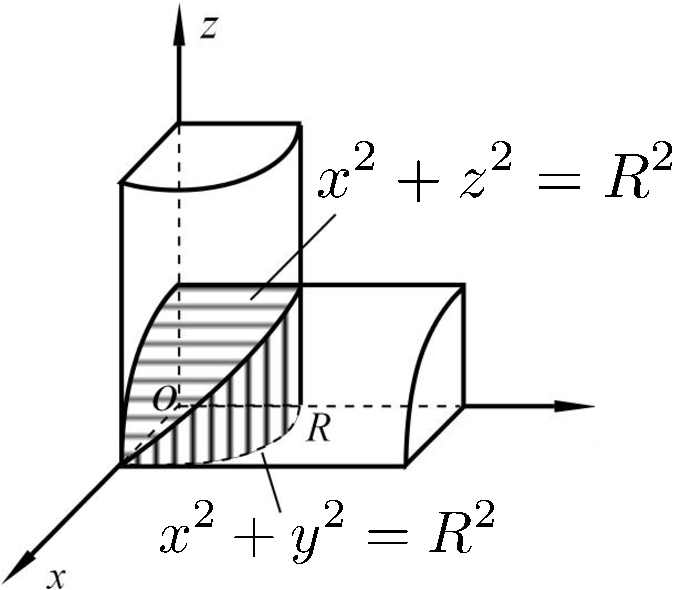
\includegraphics{./images/ch11/intersectV.pdf}}
% % 		\end{center}
% % 	\end{columns}
% % \end{frame}
% 
% \begin{frame}
% 	\linespread{1.2}
% 	\begin{exampleblock}{{\bf 例7}\hfill}
% 		计算累次积分
% 		$$I=\int_{1/4}^{1/2}\int_{1/2}^{\sqrt y}e^{y/x}dxdy+
% 		\int_{1/2}^1\int_y^{\sqrt y}e^{y/x}dxdy$$
% 	\end{exampleblock}
% \end{frame}
% 
% \begin{frame}
% 	\linespread{1.2}
% % 	\begin{columns}
% % 		\column{.5\textwidth}
% 			\begin{exampleblock}{{\bf 例8}\hfill}
% 			求两柱面$x^2+y^2=R^2,\, x^2+z^2=R^2$
% 			相交所围成的立体体积。
% 		\end{exampleblock}\pause 
% % 		\column{.5\textwidth}
% 			\begin{center}
% 			\resizebox{!}{5cm}{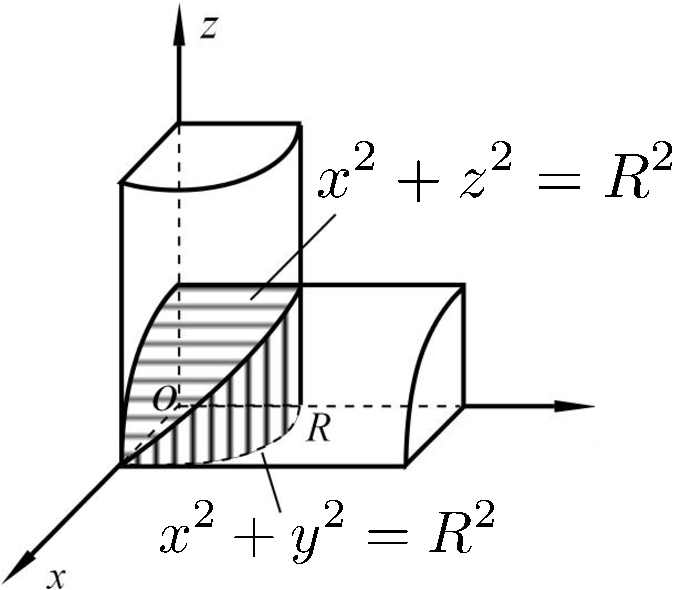
\includegraphics{./images/ch11/intersectV.pdf}}
% 		\end{center}
% % 	\end{columns}
% \end{frame}

\begin{frame}[<+->]{小结}
	\linespread{1.2}
	\begin{enumerate}
	  \item {\bf 重积分的定义:}“分割取近似,做和求极限”
	  $$\iint_Df(x,y)\d\sigma=\lim_{d(T)\to
		  0}\sum_{i=1}^nf(\xi_i,\eta_i)\Delta\sigma_i$$
	  \item {\bf 重积分的基本性质}
	  \begin{itemize}
	    \item 与定积分的性质加以类比
	  \end{itemize}
% 	  \item {\bf 二重积分与累次积分:}积分次序与积分区域的表示
% 	  $$\iint_Df(x,y)d\sigma=\int_{x_1}^{x_2}
% 	\int_{\varphi_1(x)}^{\varphi_2(x)}f(x,y)dydx$$
	\end{enumerate}
\end{frame}

%=====================================
 
% \begin{frame}{title}
% 	\linespread{1.2}
% 	\begin{exampleblock}{{\bf title}\hfill}
% 		123
% 	\end{exampleblock}
% \end{frame}
% 
% \begin{frame}{title}
% 	\linespread{1.2}
% 	\begin{block}{{\bf title}\hfill}
% 		123
% 	\end{block}
% \end{frame}